% Icon for the romda card on the Docs page of andreanovoa.github.io: the
% sequential data-assimilation cycle drawn as uncertainty tubes. Between
% observations the forecast (orange) spreads and drifts from the truth (black);
% at each observation the forecast covariance (orange oval) and the observation
% covariance (red oval) combine into the smaller analysis covariance (blue
% oval), from which the next, narrower tube starts.
% Background is left transparent so the card's dark-theme inversion blends it.
% Build: pdflatex romda.tex && pdftocairo -svg romda.pdf romda.svg
\documentclass[border=1pt]{standalone}
\usepackage{tikz}

\definecolor{truth}{HTML}{222222}
\definecolor{fc}{HTML}{EE7733}
\definecolor{an}{HTML}{0077BB}
\definecolor{ob}{HTML}{CC3311}

\def\truth#1{0.75*sin(110*(#1))}

\begin{document}
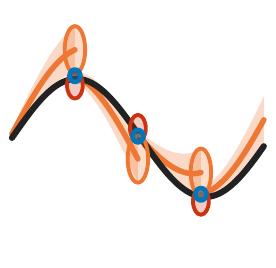
\begin{tikzpicture}[x=1cm, y=1cm, line cap=round, line join=round]
  \useasboundingbox (0.2,-1.3) rectangle (3.0,1.4);
  % forecast tubes: each starts at an analysis with offset \e from the truth,
  % drifts with slope \d, and widens linearly between observations
  \foreach \t/\e/\d in {0/0.05/0.40, 0.8/0.04/-0.45, 1.6/-0.03/0.42, 2.4/0.03/0.38} {
    \fill[fc, opacity=0.28]
      plot[domain=\t:\t+0.8, samples=20] (\x, {\truth{\x} + \e + \d*(\x-\t) + 0.06 + 0.3*(\x-\t)})
      -- plot[domain=\t+0.8:\t, samples=20] (\x, {\truth{\x} + \e + \d*(\x-\t) - 0.06 - 0.3*(\x-\t)})
      -- cycle;
    \draw[fc, line width=2pt]
      plot[domain=\t:\t+0.8, samples=20] (\x, {\truth{\x} + \e + \d*(\x-\t)});
  }
  % truth
  \draw[truth, line width=2.2pt, domain=0:3.2, samples=80] plot (\x, {\truth{\x}});
  % covariances at each observation: forecast, observation and analysis
  \foreach \t/\f/\o/\a in {0.8/0.37/-0.08/0.04, 1.6/-0.32/0.07/-0.03, 2.4/0.31/-0.06/0.03} {
    \pgfmathsetmacro{\y}{\truth{\t}}
    \draw[fc, line width=1.4pt, fill=fc, fill opacity=0.25] (\t,\y+\f) ellipse (0.13 and 0.30);
    \draw[ob, line width=1.4pt, fill=ob, fill opacity=0.25] (\t,\y+\o) ellipse (0.10 and 0.17);
    \draw[an, line width=1.6pt, fill=an, fill opacity=0.45] (\t,\y+\a) ellipse (0.07 and 0.08);
  }
\end{tikzpicture}
\end{document}
